\documentclass[journal,12pt,twocolumn]{IEEEtran}
%
\usepackage{setspace}
\usepackage{gensymb}
%\doublespacing
\singlespacing

%\usepackage{graphicx}
%\usepackage{amssymb}
%\usepackage{relsize}
\usepackage[cmex10]{amsmath}
%\usepackage{amsthm}
%\interdisplaylinepenalty=2500
%\savesymbol{iint}
%\usepackage{txfonts}
%\restoresymbol{TXF}{iint}
%\usepackage{wasysym}
\usepackage{amsthm}
%\usepackage{iithtlc}
\usepackage{mathrsfs}
\usepackage{txfonts}
\usepackage{stfloats}
\usepackage{bm}
\usepackage{cite}
\usepackage{cases}
\usepackage{subfig}
%\usepackage{xtab}
\usepackage{longtable}
\usepackage{multirow}
%\usepackage{algorithm}
%\usepackage{algpseudocode}
\usepackage{enumitem}
\usepackage{mathtools}
\usepackage{tikz}
\usepackage{circuitikz}
\usepackage{verbatim}
\usepackage{tfrupee}
\usepackage[breaklinks=true]{hyperref}
%\usepackage{stmaryrd}
\usepackage{tkz-euclide} % loads  TikZ and tkz-base
\usetkzobj{all}
\usetikzlibrary{decorations.markings}
\usetikzlibrary{shapes.geometric}
\newif\iflabrev
\usepackage{listings}
    \usepackage{color}                                            %%
    \usepackage{array}                                            %%
    \usepackage{longtable}                                        %%
    \usepackage{calc}                                             %%
    \usepackage{multirow}                                         %%
    \usepackage{hhline}                                           %%
    \usepackage{ifthen}                                           %%
  %optionally (for landscape tables embedded in another document): %%
    \usepackage{lscape}     
\usepackage{multicol}
\usepackage{chngcntr}
%\usepackage{enumerate}

%\usepackage{wasysym}
%\newcounter{MYtempeqncnt}
\DeclareMathOperator*{\Res}{Res}
%\renewcommand{\baselinestretch}{2}
\renewcommand\thesection{\arabic{section}}
\renewcommand\thesubsection{\thesection.\arabic{subsection}}
\renewcommand\thesubsubsection{\thesubsection.\arabic{subsubsection}}

\renewcommand\thesectiondis{\arabic{section}}
\renewcommand\thesubsectiondis{\thesectiondis.\arabic{subsection}}
\renewcommand\thesubsubsectiondis{\thesubsectiondis.\arabic{subsubsection}}

% correct bad hyphenation here
\hyphenation{op-tical net-works semi-conduc-tor}
\def\inputGnumericTable{}                                 %%

\lstset{
%language=C,
frame=single, 
breaklines=true,
columns=fullflexible
}
%\lstset{
%language=tex,
%frame=single, 
%breaklines=true
%}

\begin{document}
%


\newtheorem{theorem}{Theorem}[section]
\newtheorem{problem}{Problem}
\newtheorem{proposition}{Proposition}[section]
\newtheorem{lemma}{Lemma}[section]
\newtheorem{corollary}[theorem]{Corollary}
\newtheorem{example}{Example}[section]
\newtheorem{definition}[problem]{Definition}
%\newtheorem{thm}{Theorem}[section] 
%\newtheorem{defn}[thm]{Definition}
%\newtheorem{algorithm}{Algorithm}[section]
%\newtheorem{cor}{Corollary}
\newcommand{\BEQA}{\begin{eqnarray}}
\newcommand{\EEQA}{\end{eqnarray}}
\newcommand{\define}{\stackrel{\triangle}{=}}
\bibliographystyle{IEEEtran}
%\bibliographystyle{ieeetr}
\providecommand{\mbf}{\mathbf}
\providecommand{\pr}[1]{\ensuremath{\Pr\left(#1\right)}}
\providecommand{\qfunc}[1]{\ensuremath{Q\left(#1\right)}}
\providecommand{\sbrak}[1]{\ensuremath{{}\left[#1\right]}}
\providecommand{\lsbrak}[1]{\ensuremath{{}\left[#1\right.}}
\providecommand{\rsbrak}[1]{\ensuremath{{}\left.#1\right]}}
\providecommand{\brak}[1]{\ensuremath{\left(#1\right)}}
\providecommand{\lbrak}[1]{\ensuremath{\left(#1\right.}}
\providecommand{\rbrak}[1]{\ensuremath{\left.#1\right)}}
\providecommand{\cbrak}[1]{\ensuremath{\left\{#1\right\}}}
\providecommand{\lcbrak}[1]{\ensuremath{\left\{#1\right.}}
\providecommand{\rcbrak}[1]{\ensuremath{\left.#1\right\}}}
\theoremstyle{remark}
\newtheorem{rem}{Remark}
\newcommand{\sgn}{\mathop{\mathrm{sgn}}}
\providecommand{\abs}[1]{\left\vert#1\right\vert}
\providecommand{\res}[1]{\Res\displaylimits_{#1}} 
\providecommand{\norm}[1]{\left\lVert#1\right\rVert}
%\providecommand{\norm}[1]{\lVert#1\rVert}
\providecommand{\mtx}[1]{\mathbf{#1}}
\providecommand{\mean}[1]{E\left[ #1 \right]}
\providecommand{\fourier}{\overset{\mathcal{F}}{ \rightleftharpoons}}
%\providecommand{\hilbert}{\overset{\mathcal{H}}{ \rightleftharpoons}}
\providecommand{\system}{\overset{\mathcal{H}}{ \longleftrightarrow}}
	%\newcommand{\solution}[2]{\textbf{Solution:}{#1}}
\newcommand{\solution}{\noindent \textbf{Solution: }}
\newcommand{\cosec}{\,\text{cosec}\,}
\providecommand{\dec}[2]{\ensuremath{\overset{#1}{\underset{#2}{\gtrless}}}}
\newcommand{\myvec}[1]{\ensuremath{\begin{pmatrix}#1\end{pmatrix}}}
\newcommand{\mydet}[1]{\ensuremath{\begin{vmatrix}#1\end{vmatrix}}}
%\numberwithin{equation}{section}
\numberwithin{equation}{subsection}
%\numberwithin{problem}{section}
%\numberwithin{definition}{section}
\makeatletter
\@addtoreset{figure}{problem}
\makeatother
\let\StandardTheFigure\thefigure
\let\vec\mathbf
%\renewcommand{\thefigure}{\theproblem.\arabic{figure}}
\renewcommand{\thefigure}{\theproblem}
%\setlist[enumerate,1]{before=\renewcommand\theequation{\theenumi.\arabic{equation}}
%\counterwithin{equation}{enumi}
%\renewcommand{\theequation}{\arabic{subsection}.\arabic{equation}}
\def\putbox#1#2#3{\makebox[0in][l]{\makebox[#1][l]{}\raisebox{\baselineskip}[0in][0in]{\raisebox{#2}[0in][0in]{#3}}}}
     \def\rightbox#1{\makebox[0in][r]{#1}}
     \def\centbox#1{\makebox[0in]{#1}}
     \def\topbox#1{\raisebox{-\baselineskip}[0in][0in]{#1}}
     \def\midbox#1{\raisebox{-0.5\baselineskip}[0in][0in]{#1}}
\vspace{3cm}
\title{
%	\logo{
Control Systems
%	}
}
\author{ G V V Sharma$^{*}$% <-this % stops a space
	\thanks{*The author is with the Department
		of Electrical Engineering, Indian Institute of Technology, Hyderabad
		502285 India e-mail:  gadepall@iith.ac.in. All content in this manual is released under GNU GPL.  Free and open source.}
	
}	
%\title{
%	\logo{Matrix Analysis through Octave}{\begin{center}\includegraphics[scale=.24]{tlc}\end{center}}{}{HAMDSP}
%}
% paper title
% can use linebreaks \\ within to get better formatting as desired
%\title{Matrix Analysis through Octave}
%
%
% author names and IEEE memberships
% note positions of commas and nonbreaking spaces ( ~ ) LaTeX will not break
% a structure at a ~ so this keeps an author's name from being broken across
% two lines.
% use \thanks{} to gain access to the first footnote area
% a separate \thanks must be used for each paragraph as LaTeX2e's \thanks
% was not built to handle multiple paragraphs
%
%\author{<-this % stops a space
%\thanks{}}
%}
% note the % following the last \IEEEmembership and also \thanks - 
% these prevent an unwanted space from occurring between the last author name
% and the end of the author line. i.e., if you had this:
% 
% \author{....lastname \thanks{...} \thanks{...} }
%                     ^------------^------------^----Do not want these spaces!
%
% a space would be appended to the last name and could cause every name on that
% line to be shifted left slightly. This is one of those "LaTeX things". For
% instance, "\textbf{A} \textbf{B}" will typeset as "A B" not "AB". To get
% "AB" then you have to do: "\textbf{A}\textbf{B}"
% \thanks is no different in this regard, so shield the last } of each \thanks
% that ends a line with a % and do not let a space in before the next \thanks.
% Spaces after \IEEEmembership other than the last one are OK (and needed) as
% you are supposed to have spaces between the names. For what it is worth,
% this is a minor point as most people would not even notice if the said evil
% space somehow managed to creep in.
% The paper headers
%\markboth{Journal of \LaTeX\ Class Files,~Vol.~6, No.~1, January~2007}%
%{Shell \MakeLowercase{\textit{et al.}}: Bare Demo of IEEEtran.cls for Journals}
% The only time the second header will appear is for the odd numbered pages
% after the title page when using the twoside option.
% 
% *** Note that you probably will NOT want to include the author's ***
% *** name in the headers of peer review papers.                   ***
% You can use \ifCLASSOPTIONpeerreview for conditional compilation here if
% you desire.
% If you want to put a publisher's ID mark on the page you can do it like
% this:
%\IEEEpubid{0000--0000/00\$00.00~\copyright~2007 IEEE}
% Remember, if you use this you must call \IEEEpubidadjcol in the second
% column for its text to clear the IEEEpubid mark.
% make the title area
\maketitle
\newpage
\tableofcontents
\bigskip
\renewcommand{\thefigure}{\theenumi}
\renewcommand{\thetable}{\theenumi}
%\renewcommand{\theequation}{\theenumi}
%\begin{abstract}
%%\boldmath
%In this letter, an algorithm for evaluating the exact analytical bit error rate  (BER)  for the piecewise linear (PL) combiner for  multiple relays is presented. Previous results were available only for upto three relays. The algorithm is unique in the sense that  the actual mathematical expressions, that are prohibitively large, need not be explicitly obtained. The diversity gain due to multiple relays is shown through plots of the analytical BER, well supported by simulations. 
%
%\end{abstract}
% IEEEtran.cls defaults to using nonbold math in the Abstract.
% This preserves the distinction between vectors and scalars. However,
% if the journal you are submitting to favors bold math in the abstract,
% then you can use LaTeX's standard command \boldmath at the very start
% of the abstract to achieve this. Many IEEE journals frown on math
% in the abstract anyway.
% Note that keywords are not normally used for peerreview papers.
%\begin{IEEEkeywords}
%Cooperative diversity, decode and forward, piecewise linear
%\end{IEEEkeywords}
% For peer review papers, you can put extra information on the cover
% page as needed:
% \ifCLASSOPTIONpeerreview
% \begin{center} \bfseries EDICS Category: 3-BBND \end{center}
% \fi
%
% For peerreview papers, this IEEEtran command inserts a page break and
% creates the second title. It will be ignored for other modes.
%\IEEEpeerreviewmaketitle
\begin{abstract}
This manual is an introduction to control systems based on GATE problems.Links to sample Python codes are available in the text.  
\end{abstract}
Download python codes using 
\begin{lstlisting}
svn co https://github.com/gadepall/school/trunk/control/codes
\end{lstlisting}
%\section{Mason's Gain Formula}
%\section{Bode Plot}
%\subsection{Introduction}
%\subsection{Example}
%\section{Second order System}
%\subsection{Damping}
%\subsection{Example}
%\section{Routh Hurwitz Criterion}
%\subsection{Routh Array}
%\subsection{Marginal Stability}
%\subsection{Stability}
%\input{./chapters/EE18BTECH11021.tex}
%\section{State-Space Model}
%\input{./chapters/ee18btech11004.tex}
%\subsection{Second Order System}
%\section{Nyquist Plot}
%\section{Phase Margin}
%\section{Gain Margin}
%\section{Compensators}
%\subsection{Phase Lead}
%\input{./chapters/EE18BTECH11021_2.tex}
%\section{Oscillator}
\section{Lag-Lead Compensator Designing}
\begin{enumerate}[label=\thesubsection.\arabic*.,ref=\thesubsection.\theenumi]
\numberwithin{equation}{enumi}
\item Using the frequency response method, design a lag-lead compensator for the unity feedback system given 
\begin{align}
G(S) = \frac{K(s+7)}{s(s+5)(s+15)}
\end{align}
The following specifications must be met: Peak overshoot = 15\%, settling time = 0.1 second and velocity error constant = 1000
Use second order approximation. \\
%
\solution Figure: \ref{fig:1;} models the equivalent of compensated closed loop system. 
\begin{figure}[!ht]
\begin{center}
		\resizebox{\columnwidth}{!}{
}
\end{center}
\caption{}
\label{fig:1;}
\end{figure}
%
Velocity error constant  
\begin{align}
K_{v} &=  \lim_{s \to 0}sG(s)
\end{align}
\begin{align}
\lim_{t \to 0}s\frac{K(s+7)}{s(s+5)(s+15)} &= 1000
\end{align}
\begin{align}
\implies K &= 10714
\end{align}
Bode plot of G(s) for the value of K
%%
\begin{figure}[!ht]
\centering
  \includegraphics[width=\columnwidth]{./figs/ee18btech11012/ee18btech11012_1.eps}
\caption{}
\label{fig:ee18btech11012}
\end{figure}
%%
The following code verifies the result.
\begin{lstlisting}
codes/ee18btech11012/ee18btech11012_1.py
\end{lstlisting}
Relation between \%OS and Damping ratio
\begin{align}
\zeta &= \frac{-\ln(\%OS/100)}{\sqrt{(\pi)^2 + (\ln(\%OS/100))^2}}
\end{align}
\begin{align}
\implies\zeta &= 0.517 
\end{align}
Phase Margin for a Damping ratio is given by
\begin{align}
\phi_{m} &= 90\degree - \arctan(\frac{\sqrt{-2\zeta^2+\sqrt{1+4\zeta^4}}}{2\zeta}
\end{align}
\begin{align}
\implies \phi_{m} &= 53.17\degree
\end{align}
For an additional 5\degree for lag compensation,Phase margin is
\begin{align}
    \phi_{m} &= 53.17\degree + 5\degree= 58.17\degree
\end{align}
\textbf{Note} : Adding 5\degree phase angle to compensate the phase angle contribution of the lag compensator.
Bandwidth frequency is given by
\begin{align}
\omega_{BW} &= \omega_{n}(\sqrt{(1-2\zeta^2)+\sqrt{4\zeta^4-4\zeta^2+2}})
\end{align}
where
\begin{align}
    \omega_{n} &= \frac{4}{T_{s}\zeta}
\end{align}
Given settling time = 0.1 sec then 
\begin{align}
    \omega_{n} &= 77.37 rad/sec 
\end{align}
then
\begin{align}
    \omega_{BW} &= 96.91 rad/sec
\end{align}
\item Designing Lag-Lead Compensator Gc(s) \\
\solution 
General lag-lead compensator 
\begin{align}
G_{c}(s) &= \left(\frac{s+\frac{1}{T_1}}{s+\frac{\gamma}{T_1}}\right)\left(\frac{s+\frac{1}{T_2}}{s+\frac{1}{\gamma T_2}}\right) 
\end{align}
\begin{itemize}
\item Choose the new phase-margin frequency 
\begin{align}
    \omega_{Pm} &= 0.8 \omega_{BW} &= 77.53 rad/sec
\end{align}
\item At this phase-margin frequency,Phase angle is -170.52\degree.
\item Then the conribution required from the lead is
\begin{align}
    \phi_{max} &= 58.17-(180-170.52)=48.69\degree.
\end{align}

\item Now Using the relation 
\begin{align}
    \phi_{max} &= \sin^{-1}(\frac{1-\beta}{1+\beta})
\end{align}
then we get
\begin{align}
    \beta &= 0.142
\end{align}
\item \underline{Lag Compensator Design}:The Compensator must have a dc gain of unity to retain the value of Kv that we have already designed by setting K = 10714.
\begin{align}
    z_{clag} &= \frac{\omega_{Pm}}{10}=\frac{77.53}{10}=7.753
\end{align}
\begin{align}
    p_{clag} &= z_{clag}*\beta=1.102
\end{align}
Gain in the lag compensator is 
\begin{align}
    K_{clag} &= \frac{p_{clag}}{z_{clag}}=0.1421
\end{align}
\item Hence the lag compensator transfer function is
\begin{align}
 G_{clag}(s) &= \frac{0.1421(s+7.753)}{s+1.102} 
\end{align}
\item \underline{Lead Compensator Design}:DC gain for this must be unity.

\textbf{Relations to find T and $\beta$}:
The Compensator's magnitude at the phase margin frequency $\omega_{max}$
\begin{align}
     |G_{c}(j\omega_{max})| &= \frac{1}{\sqrt{\beta}} 
\end{align}
\begin{align}
    T &= \frac{1}{\omega_{max}\sqrt{\beta}}
\end{align}
So,To find transfer function
\begin{align}
    z_{lead} &= \frac{1}{T_{2}}=\omega_{Pm}*\sqrt{\beta}=29.92
\end{align}
\begin{align}
    p_{lead} &= \frac{z_{lead}}{\beta}=205.74,K_{lead}=\frac{p_{lead}}{z_{lead}}=7.04
\end{align}
\item Thus lead compensator transfer function is 
\begin{align}
    G_{lead} &= \frac{7.04(s+29.22)}{s+205.74} 
\end{align}
\item So the overall compensator tranfer function is
\begin{align}
    G_{c}(s) &= G_{clag}(s)G_{lead}(s)
\end{align}
\begin{align}
G_{c}(s)&=\frac{1.000384(s+7.753)(s+29.23)}{(s+1.102)(s+205.7)}
\end{align}
\end{itemize}
\item Verifying Lag-lead Compensator using Plots \\
\solution 
Magnitude and Phase plot
\begin{figure}[!ht]
\centering
  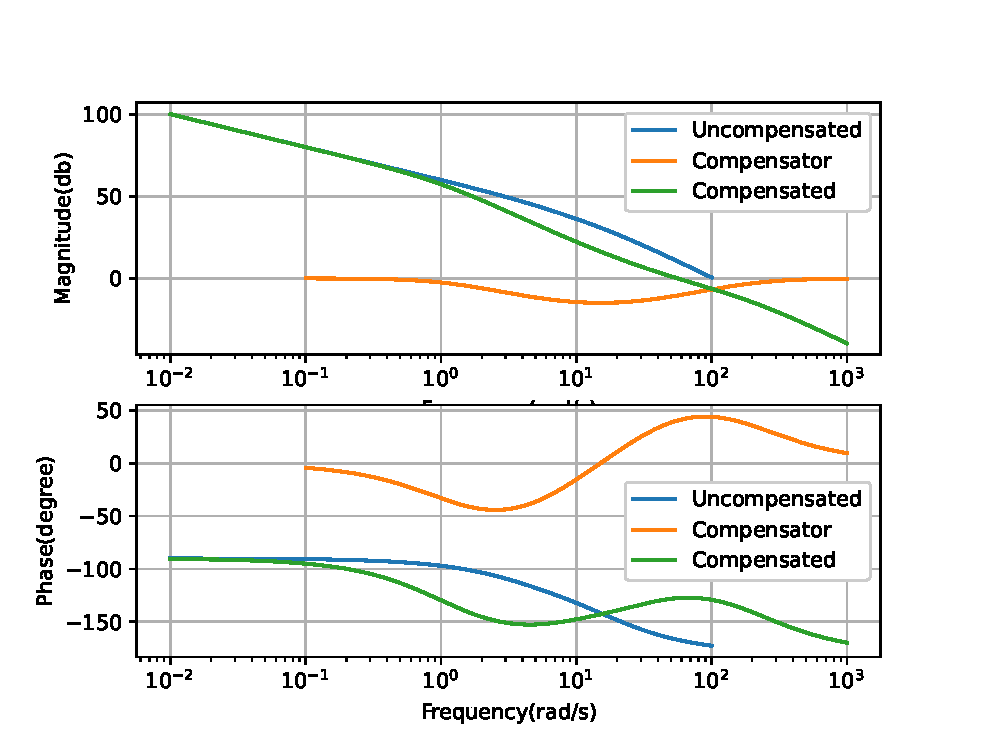
\includegraphics[width=\columnwidth]{./figs/ee18btech11012/ee18btech11012_2.eps}
\caption{}
\label{fig:ee18}
\end{figure}
The following code 
\begin{lstlisting}
codes/ee18btech11012/ee18btech11012_2.py
\end{lstlisting}
\item Verifying in time domain \\
\solution 
Time response for a unit step function
\begin{figure}[!ht]
\centering
  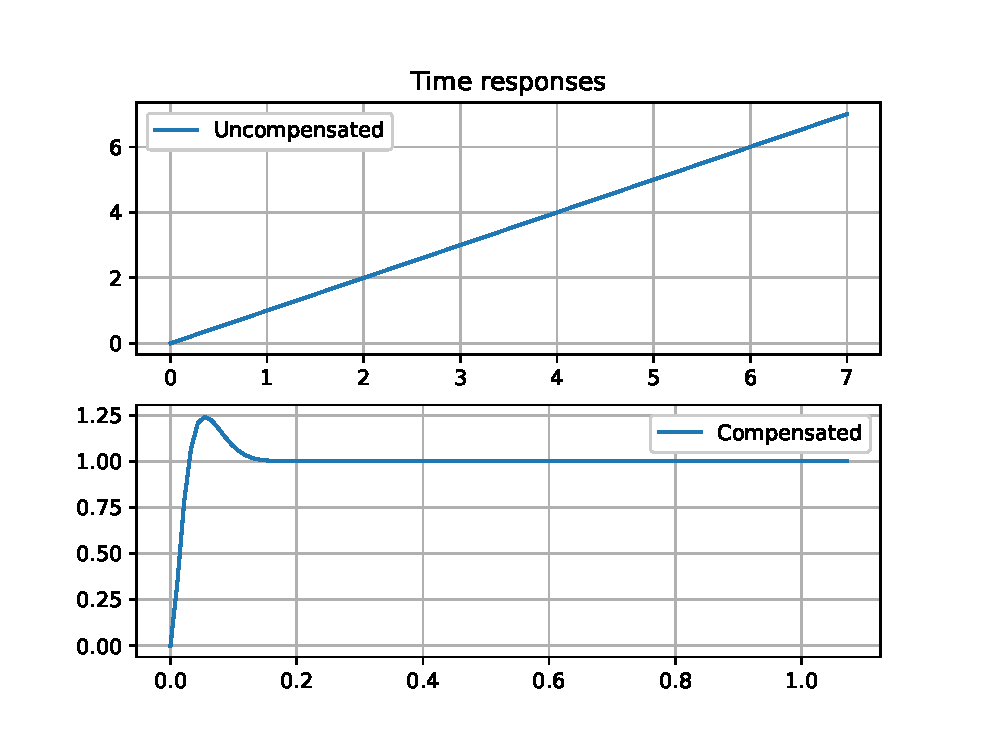
\includegraphics[width=\columnwidth]{./figs/ee18btech11012/ee18btech11012_3.eps}
\caption{}
\label{fig:2} 
\end{figure}
The following code can be verified
\begin{lstlisting}
codes/ee18btech11012/ee18btech11012_3.py
\end{lstlisting}
\item Verifying the designed lag-lead compensator \\
\solution 
\begin{table}[!ht]
\centering


\caption{Comparing the desired and obtained results}
\label{table:ee18btech11012_table1}
\end{table}
\end{enumerate}

\end{document}
